\documentclass[../../relatorio.tex]{subfiles}
\begin{document}
Neste subsistema podem encontrar-se funcionalidades relacionadas com as \textbf{Reparações}. 
Este, por sua vez, está dividido em 3 \textit{packages}:
\begin{itemize}
    \item [Orçamento]{
                    Responsável por atribuir um orçamento a um equipamento. 
                    Aqui, verifica-se que o orçamento tem um estado, facilitando o processo e dando um ponto de situação sobre o mesmo. 
                    Está também associado ao \textit{package} plano de trabalho, sendo gerado a partir deste, e a uma comunicação, que tem como função 
                    interagir com o cliente se necessário.
                    É de salientar a relação com um outro subsistema, SSClientes, devido ao atributo do equipamento. 
                    }
    \item [Reparação]{
                    Responsável pela reparação do equipamento. Existem dois tipos de reparação: Reparação Programada e a Reparação Expresso. Cada reparação tem um estado, de forma 
                    a facilitar o processo e dando um ponto de situação, e está associado a um orçamento, a um plano de trabalhos e a uma lista de comunicações que serão feitas, caso sejam feitas,
                    com o cliente. É de salientar a existência da classe ReparacoesPorMes, na medida que esta foi criada a facilitar as listagens dos colaboradores.
                    } 
    \item [Plano de Trabalho]{
                    Responsável pelo planeamento dos passos e subpassos de uma reparação. 
                    Aqui, verifica-se que o plano de trabalhos tem como atributos duas listas distintas de passos de reparação. Por sua vez, esta classe, passo de reparação,
                    está associada ao material. 
                    A classe material representa todos os materias usados pelo passo de reparação, ou seja, é impossível categorizar um conjunto 
                    variado de materiais, porém, a classe CategoriaMaterial encontra-se presente na mesma, sendo que, é uma possível melhoria neste trabalho, isto é, 
                    a classe Material passaria a representar não um conjunto de materiais, mas apenas um, ao qual estaria associado uma categoria. Daqui também se poderia aprofundar
                    a ideia do stock da loja. 
                    }
\end{itemize}


\subsection{GestReparaçõesFacade}
Esta classe é responsável por toda a gestão das reparações e funcionalidades, implementando a interface IGestReparacoes.

Analisando os métodos que esta classe implementa, identificou-se que, para melhorar a navegabilidade
e a \textit{performance} do sistema, será necessário que este tenha um conjunto de atributos, nomeadamente:
\begin{itemize}
    \item [reps]{Map de Reparações que podem ser acessidas através do seu ID}
    \item [reparacoesDisponiveis]{Set de Reparacoes Expresso}
    \item [orcs]{Mapa de Orçamentos que podem ser acessidos através do seu ID}
\end{itemize}



\begin{figure}[!ht]
    \centering
    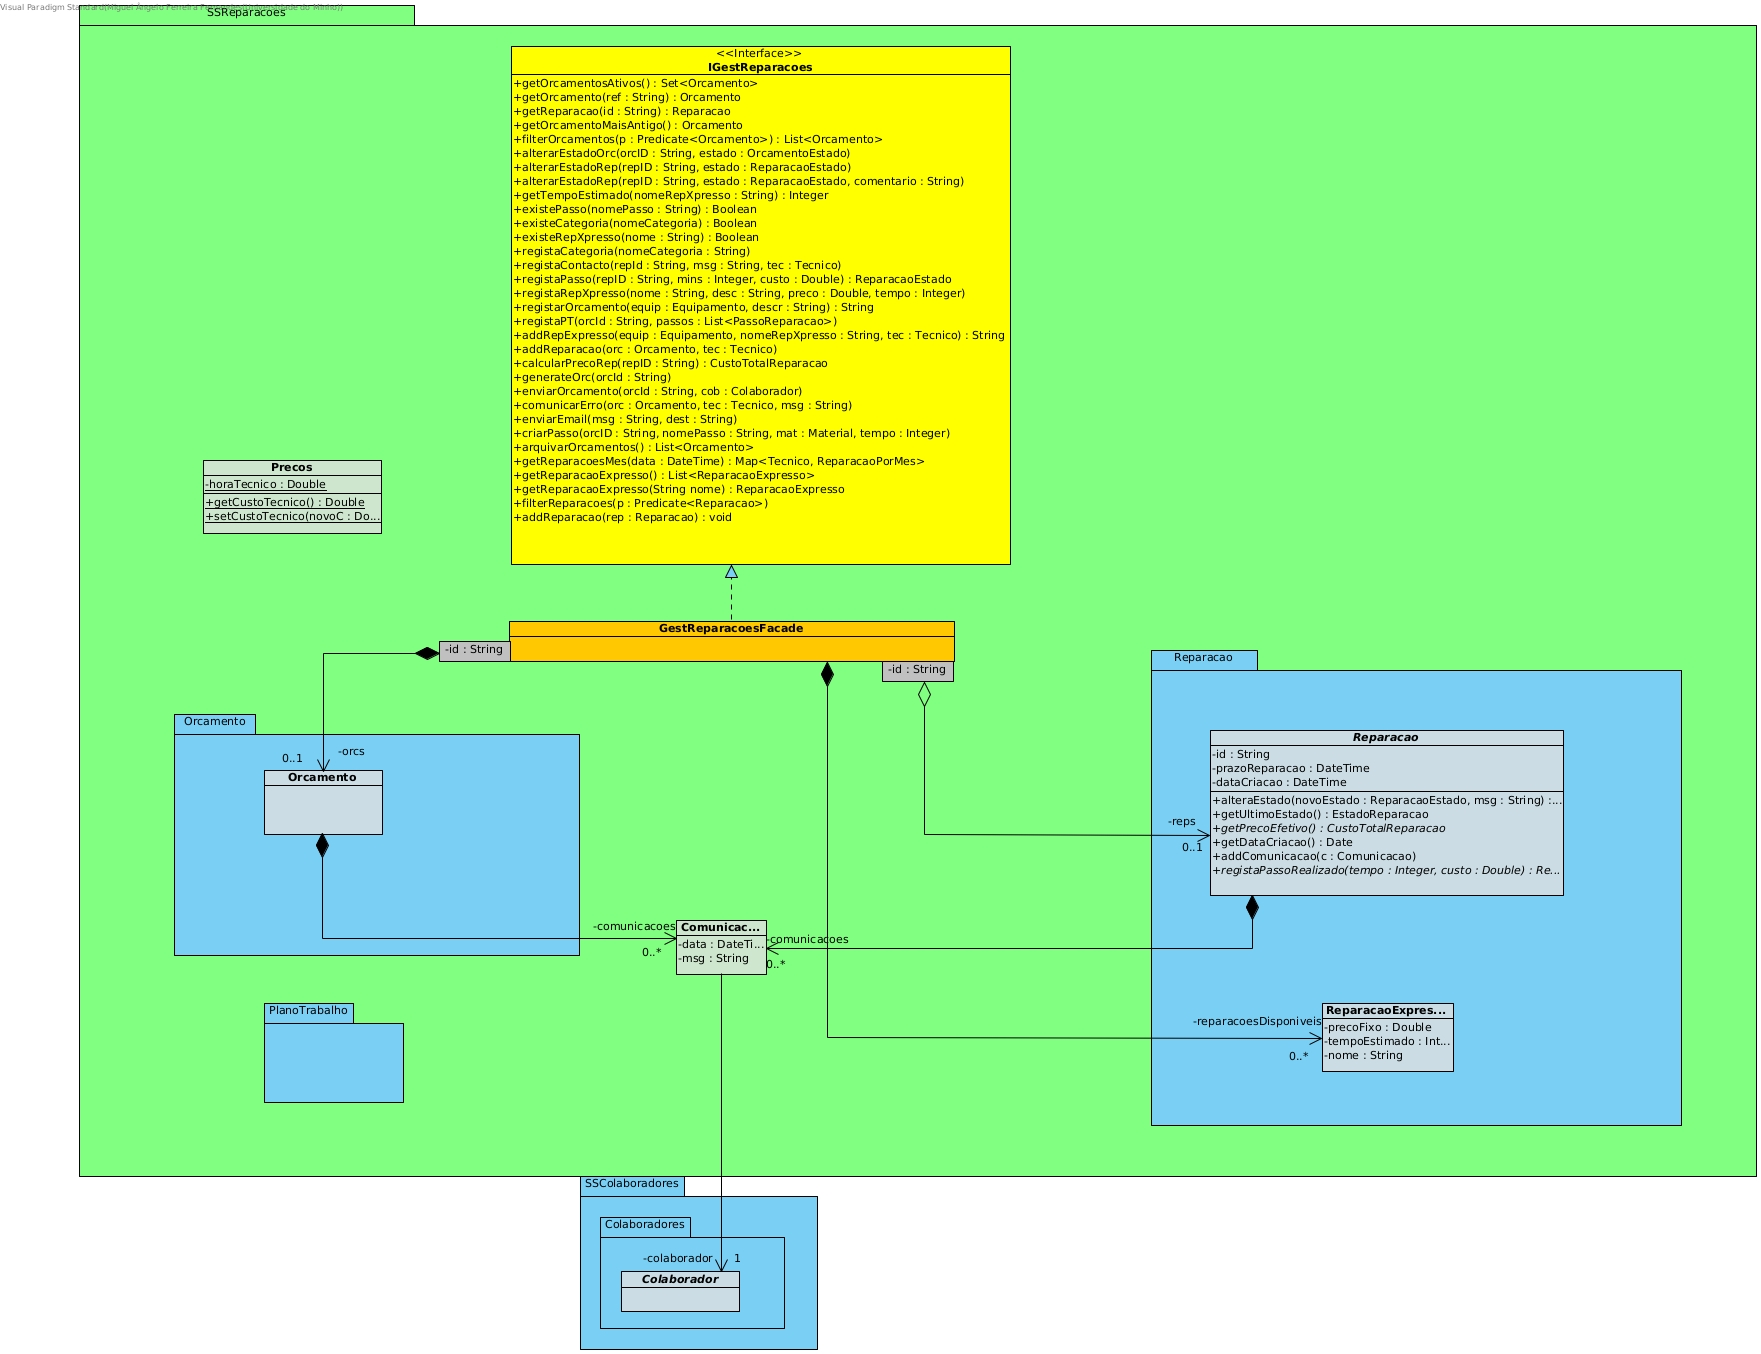
\includegraphics[scale=0.27]{SSReparacoesPackage.jpg}
    \caption{SubSistema SSReparacoes \ref{sec:ss_reparacoes}}
\end{figure}
\end{document}